% Compiled with plain pdflatex + pdfcrop (the `standalone` class is not
% installed in this TeX distribution), so the page is cropped to the
% diagram's bounding box after compilation -- see build instructions below.
\documentclass{article}
\usepackage[paperwidth=45cm, paperheight=20cm, margin=0cm]{geometry}
\usepackage{tikz}
\usetikzlibrary{positioning, arrows.meta, shapes.geometric, calc, shapes.misc}
\pagestyle{empty}
\setlength{\parindent}{0pt}

\begin{document}

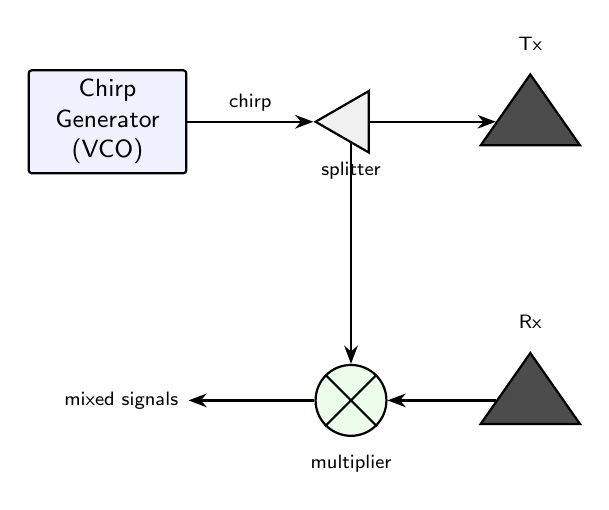
\begin{tikzpicture}[
    font=\sffamily\small,
    >=Latex,
    thick,
    block/.style={
        draw, rounded corners=1pt, minimum height=1cm, minimum width=2cm,
        align=center, fill=blue!6
    },
    mixer/.style={
        draw, circle, minimum size=0.9cm, fill=green!8
    },
    splitter/.style={
        draw, regular polygon, regular polygon sides=3,
        shape border rotate=90, minimum size=0.9cm, fill=gray!12
    },
    antenna/.style={
        draw, isosceles triangle, isosceles triangle apex angle=70,
        shape border rotate=90, minimum height=0.9cm, minimum width=0.9cm,
        fill=black!70, draw=black
    },
    arrowlabel/.style={font=\scriptsize\sffamily, midway, above},
    >=Stealth
]

    % ---------- Transmit chain ----------
    \node[block] (vco) {Chirp\\Generator\\(VCO)};
    \node[splitter, right=1.6cm of vco] (split) {};
    \node[antenna, right=1.6cm of split] (txant) {};

    \node[above=0.15cm of txant, font=\scriptsize\sffamily] {Tx};
    \node[below=0.1cm of split, font=\scriptsize\sffamily] {splitter};

    % ---------- Receive chain ----------
    \node[antenna, below=2.6cm of txant] (rxant) {};
    \node[mixer] (mix) at (split |- rxant) {};

    \node[above=0.15cm of rxant, font=\scriptsize\sffamily] {Rx};
    \node[below=0.1cm of mix, font=\scriptsize\sffamily] {multiplier};

    % ---------- Output ----------
    \node[left=1.6cm of mix, align=center, font=\scriptsize\sffamily] (out) {mixed signals};

    % ---------- Connections: transmit path ----------
    \draw[->] (vco) -- node[arrowlabel] {chirp} (split);
    \draw[->] (split) -- (txant);

    % ---------- Connections: receive path ----------
    \draw[->] (rxant) -- (mix);
    \draw[->] (mix) -- (out);

    % ---------- Reference feed from splitter into mixer ----------
    \draw[->] (split) -- (mix);

    % ---------- Mixer symbol ----------
    \draw (mix.north west) -- (mix.south east);
    \draw (mix.north east) -- (mix.south west);

\end{tikzpicture}

\end{document}
